\documentclass[11pt,a4paper]{report}

\usepackage[utf8]{inputenc}
\usepackage[T1]{fontenc}
\usepackage[danish]{babel}
\usepackage[a4paper,margin=2.5cm]{geometry}
\usepackage{amsmath}
\usepackage{graphicx}
\usepackage{float}
\usepackage{booktabs}
\usepackage{listings}
\usepackage{xcolor}
\usepackage{hyperref}
\usepackage{caption}

\definecolor{codebg}{RGB}{245,245,245}
\lstset{
    backgroundcolor=\color{codebg},
    basicstyle=\ttfamily\small,
    breaklines=true,
    frame=single,
    numbers=left,
    numberstyle=\tiny,
    keywordstyle=\color{blue},
    commentstyle=\color{gray},
    showstringspaces=false,
    columns=fullflexible,
    inputencoding=utf8,
    extendedchars=true,
    literate={æ}{{\ae}}1 {ø}{{\o}}1 {å}{{\aa}}1 {Æ}{{\AE}}1 {Ø}{{\O}}1 {Å}{{\AA}}1 {é}{{\'e}}1 {–}{{--}}1 {‘}{{'}}1 {’}{{'}}1
}

\setlength{\parindent}{0pt}
\setlength{\parskip}{0.5em}
\setcounter{tocdepth}{1}

% Show section numbers without chapter prefix (1, 2, 3, ...)
\renewcommand{\thesection}{\arabic{section}}

\title{\vspace{1cm}\Huge Miniprojekt A\\[0.3cm]\Large DEL 1}
\author{\textbf{Navn: Asger Grundtdal Stidsen} \\ \textbf{AU-ID: au798909} \\ \textbf{Afleveringsdato: \today}}
\date{}

\begin{document}

\maketitle

\section*{Introduktion}
\addcontentsline{toc}{section}{Introduktion}
Dette miniprojekt omhandler f\o rste del af kurset Digital Signalbehandling, hvor der er udleveret tre lydfiler, Signal 1, Signal 2 og Signal 3. Form\aa let med projektet er at analysere og behandle lydsignalerne med udgangspunkt i den teori, der er gennemg\aa et i f\o rste del af kurset.

Projektet best\aa r af i alt 10 opgaver, hvor de tre signaler anvendes til forskellige former for analyse og signalbehandling. Opgaverne omhandler blandt andet forskellige aspekter af sampling, signal- og frekvensanalyse samt behandling af lydsignaler. Den relevante teori vil blive anvendt til at forklare de udf\o rte metoder og resultater.

\tableofcontents

\clearpage
\setcounter{page}{1}

% Start sections at 0 so "Global Code" becomes section 0
\setcounter{section}{-1}

\section{Global Code}
Opgaven er lavet i Python. Nedenfor ses de biblioteker, der bruges gennem hele rapporten, samt indlæsning af de tre lydsignaler.

\begin{lstlisting}[language=Python]
import numpy as np
import matplotlib.pyplot as plt
import sympy as sym
import scipy as sci
import pandas as pd
import soundfile as sf
from IPython.display import Audio, display


# Load audio files
audio_s1, fs_s1 = sf.read("./Signal_s1.mp3")
audio_s2, fs_s2 = sf.read("./Signal_s2.mp3")
audio_s3, fs_s3 = sf.read("./Signal_s3.mp3")

f_s = 44100
t_s = 1/f_s
\end{lstlisting}

\newpage

%opgave 1
\section{Opgave: Find antal samples N for alle tre signaler}

\subsection{Forberedelse}
Når vi loader lydfilen ind i Python, har den dimensionen (N : 2). Det betyder, at den indeholder (N) samples, hvor hver sample består af en venstre og en højre lydkanal. Målet er at finde antallet af samples. Dette kan gøres med funktionen len(x) med x værende den loaded lyd.

\subsection{Kode}
\begin{lstlisting}[language=Python]
N_s1 = len(audio_s1)
N_s2 = len(audio_s2)
N_s3 = len(audio_s3)


print(f"Der er {N_s1} samples i s1")
print(f"Der er {N_s2} samples i s2")
print(f"Der er {N_s3} samples i s3")
\end{lstlisting}

\subsection{Resultat}
Kørsel af koden gav følgende antal samples:

\begin{lstlisting}[language=Bash]
    Der er 4586112 samples i s1
    Der er 9527040 samples i s2
    Der er 1382400 samples i s3
\end{lstlisting}

\subsection{Diskussion og konklusion}
Her kan vi se, at der er flest samples i signal 2, hvilket også stemmer overens med lydfilens længde på tre minutter, hvor de to andre signaler er på henholdsvis et et halvt minut og et halvt minut.

\newpage
%opgave 2
\section{Opgave: Plot alle tre signaler med korrekte tidsakser}
\subsection{Opgavebeskrivelse}
Plot alle tre signaler med korrekte tidsakser, og sæt ‘xlabel’, ‘ylabel’ og ‘title’ på

\subsection{Forberedelse}
Hvert sample i signalet har ikke en fastlagt tid. Ved at plotte samples direkte vil den korrekte tidsakse derfor ikke være repræsenteret. Derfor skal der oprettes en tidsakse, som angiver, på hvilket tidspunkt hvert sample er blevet samplet. Dette gøres ved hjælp af et index-array, som multipliceres med tiden mellem hvert sample.

Det er også her vigtigt at pointere, at signal 2 er stereo. Så den har to separate kanaler med forskellig lyddata. Dermed skal hver kanal plottes for at få alt dataen plottet.
\subsection{Kode}
\begin{lstlisting}[language=Python]
#get tid for hver sample
t_s1 = np.arange(N_s1)*t_s
t_s2 = np.arange(N_s2)*t_s
t_s3 = np.arange(N_s3)*t_s

#function til at plotte et et lyd array
def plotAudio(title_,t,a):
    plt.plot(t,a)
    plt.xlabel("Tid Sek")
    plt.ylabel("Amplityde")
    plt.title(title_)
    plt.show()
    
# plot de tre signaler
plotAudio("signal 1",t_s1,audio_s1[:,0])
plotAudio("signal 2 channel 1",t_s2,audio_s2[:,0])
plotAudio("signal 2 channel 2",t_s2,audio_s2[:,1])
plotAudio("signal 3",t_s3,audio_s3[:,0])
\end{lstlisting}

\subsection{Resultat}

\begin{figure}[H]
    \centering
    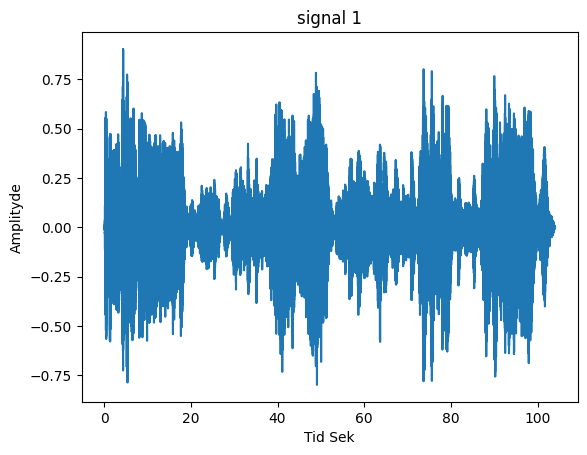
\includegraphics[width=0.8\textwidth]{images/o2_s1.png}
    \caption{Plot af signal 1}
    \label{fig:o2_s1}
\end{figure}
\begin{figure}[H]
    \centering
    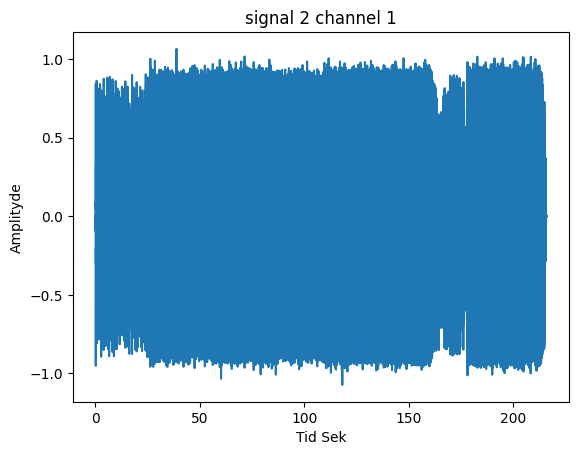
\includegraphics[width=0.8\textwidth]{images/o2_s2_c1.png}
    \caption{Plot af signal 2 kanal 1}
    \label{fig:o2_s2_c1}
\end{figure}
\begin{figure}[H]
    \centering
    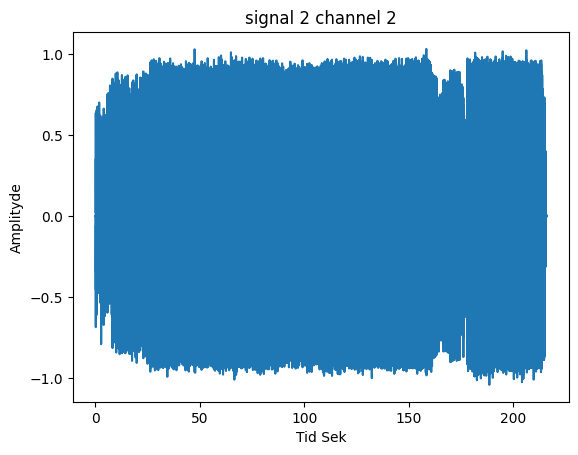
\includegraphics[width=0.8\textwidth]{images/o2_s2_c2.png}
    \caption{Plot af signal 2 kanal 2}
    \label{fig:o2_s2_c2}
\end{figure}
\begin{figure}[H]
    \centering
    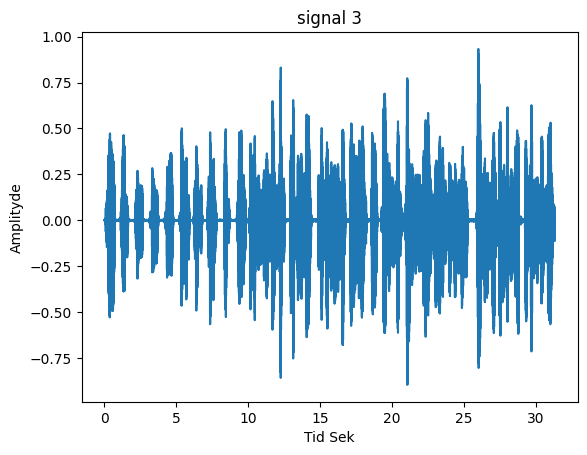
\includegraphics[width=0.8\textwidth]{images/o2_s3.png}
    \caption{Plot af signal 3}
    \label{fig:o2_s3}
\end{figure}

\subsection{Diskussion og konklusion}
vi kan se at signalerne er meget forskellige fra hinanden. Signal 2 på \autoref{fig:o2_s2_c1} har meget tætte og jævne amplitudeudsving, mens signal 3 på \autoref{fig:o2_s3} har større mellemrum mellem amplitudeudsvingene. Signal 1 på \autoref{fig:o2_s1} ligger mellem de to, hvor amplitudeudsvingene er mindre tætte end i signal 2, men tættere end i signal 3.

Derudover kan vi se, at signal 2 ikke er ens på begge kanaler. Dette stemmer overens med, at signal 2 er et stereosignal og derfor indeholder en venstre og en højre kanal, som ikke nødvendigvis har samme amplituder. Forskellen mellem kanalerne ses ved sammenligning af \autoref{fig:o2_s2_c1} og \autoref{fig:o2_s2_c2}.

\newpage

%opgave 3
\section{Opgave: Find for alle tre signaler: max, min, gennemsnit (mean), rms og effekt}

\subsection{Forberedelse}
Ved benyttelse af biblioteket NumPy er mange af disse værdier, der skal findes, allerede en indbygget funktion. Her vil der kun blive implementeret en funktion til at finde RMS-værdien og effekten. Alt dette er forholdsvis lige til og kræver ikke yderligere forklaring. Dog er det vigtigt at pointere, at signal 2 er stereo, og dermed er det vigtigt at inkludere hele signalet. Derfor vil kanal 2 blive lagt bagefter kanal 1 for at lave ét langt lydsignal, som vil give maks., min., median, RMS og effekten over alt dataen.

\subsection{Kode}
\begin{lstlisting}[language=Python]
#max
max_s1 = np.max(audio_s1[:,0])
max_s2 = np.max([audio_s2[:, 0], audio_s2[:, 1]])
max_s3 = np.max(audio_s3[:,0])

#min
min_s1 = np.min(audio_s1[:,0])
min_s2 = np.min([audio_s2[:, 0], audio_s2[:, 1]])
min_s3 = np.min(audio_s3[:,0])

#mean
mean_s1 = np.mean(audio_s1[:,0])
mean_s2 = np.mean([audio_s2[:, 0], audio_s2[:, 1]])
mean_s3 = np.mean(audio_s3[:,0])

#rms
def rms(signal):
    s = np.pow(signal,2)
    ms = np.mean(s)
    rms = np.sqrt(ms)
    return rms

rms_s1 = rms(audio_s1[:,0])
rms_s2 = rms([audio_s2[:, 0], audio_s2[:, 1]])
rms_s3 = rms(audio_s3[:,0])


#effekt
def e(signal):
    s = np.pow(signal,2)
    ms = np.mean(s)
    return ms

e_s1 = e(audio_s1[:,0])
e_s2 = e([audio_s2[:, 0], audio_s2[:, 1]])
e_s3 = e(audio_s3[:,0])

print(f"signal 1:")
print(f"max: {max_s1:.3f}")
print(f"min: {min_s1:.3f}")
print(f"mean: {mean_s1:.3e}")
print(f"rms: {rms_s1:.3f}")
print(f"effekt: {e_s1:.3e}")
print()
print(f"signal 2:")
print(f"max: {max_s2:.3f}")
print(f"min: {min_s2:.3f}")
print(f"mean: {mean_s2:.3e}")
print(f"rms: {rms_s2:.3f}")
print(f"effekt: {e_s2:.3e}")
print()
print(f"signal 3:")
print(f"max: {max_s3:.3f}")
print(f"min: {min_s3:.3f}")
print(f"mean: {mean_s3:.3e}")
print(f"rms: {rms_s3:.3f}")
print(f"effekt: {e_s3:.3e}")
print()
\end{lstlisting}

\subsection{Resultat}
\begin{lstlisting}[language=Bash]
signal 1:
max: 0.903
min: -0.798
mean: -4.102e-05
rms: 0.116
effekt: 1.352e-02

signal 2:
max: 1.064
min: -1.073
mean: -1.032e-05
rms: 0.337
effekt: 1.133e-01

signal 3:
max: 0.933
min: -0.897
mean: -5.575e-04
rms: 0.089
effekt: 7.955e-03
\end{lstlisting}

\subsection{Diskussion og konklusion}
Ud fra resultatet kan det observeres, at der er større effekt og rms i signal 2 end i signal 1 og 3. Dette stemmer også overens med det forventede. Vi kan se i \autoref{fig:o2_s2_c1}, at signalet har en større amplitude over en større del af tiden end fx. signalet i \autoref{fig:o2_s1}, hvor signalet ikke er lige så tæt og højt i amplituden.


\newpage
%opgave 4
\section{Opgave: Find de tre signalers crest-faktorer, - sammenlign og kommenter}

\subsection{Forberedelse}
Crest factor beregnes som forholdet mellem signalets peak-værdi og RMS-værdi ved hjælp af formlen $20 \log_{10}\left(\frac{x_{\text{peak}}}{x_{\text{RMS}}}\right)$. Peak-værdien er den maksimale absolutte amplitude i signalet. Derfor vil der først blive beregnet peak-værdien for de tre signaler, hvorefter disse værdier sammen med RMS-værdierne, fra opgave 3, kan indsættes i formlen for crest factor.

\subsection{Kode}
\begin{lstlisting}[language=Python]
#function til at beregne crest factor
def crest_factor(peak,rms):
    return 20*np.log10(peak/rms)

#beregn peak
peak_s1 = np.max([max_s1,-min_s1])
peak_s2 = np.max([max_s2,-min_s2])
peak_s3 = np.max([max_s3,-min_s3])

#beregne crest factor
c_s1 = crest_factor(peak_s1,rms_s1)
c_s2 = crest_factor(peak_s2,rms_s2)
c_s3 = crest_factor(peak_s3,rms_s3)

#print resultat
print("crest_factor:")
print(f"signal 1: {c_s1:.2f}")
print(f"signal 2: {c_s2:.2f}")
print(f"signal 3: {c_s3:.2f}")
\end{lstlisting}

\subsection{Resultat}
\begin{lstlisting}[language=Bash]
crest_factor:
signal 1: 17.81
signal 2: 10.07
signal 3: 20.40
\end{lstlisting}

\subsection{Diskussion og konklusion}
Resultatet viser, at signal 2 har den laveste crest factor på 10,07, efterfulgt af signal 1 på 17,81, mens signal 3 har den højeste crest factor på 20,40. Det stemmer godt overens med observationerne fra de tre figurer. I signal 2 i \autoref{fig:o2_s2_c1} kan der observeres en forholdsvis jævn og høj amplitude uden tydelige amplitudespidser, hvilket resulterer i en lavere crest factor. \autoref{fig:o2_s3} der viser Signal 3 er derimod opbyggede af mange korte og tydelige amplitudespidser, hvilket giver en større forskel mellem peak og RMS og dermed en højere crest factor. Signal 1 på i \autoref{fig:o2_s1} ligger mellem de to signaler, hvor der kan observeres bredere amplitudespidser, men uden de samme korte og markante spidser som i signal 3. Dette stemmer godt overens med de beregnede crest factor-værdier for de tre signaler.


\newpage
%opgave 5
\section{Opgave: Nedsampel s1 med en faktor 4. Plot – og sammenlign med originalen}

\subsection{Forberedelse}
Til denne opgave, hvor signalet skal downsampleres med en faktor på 4, vil funktionen decimate blive anvendt. Funktionen bruger et filter før downsampling, hvilket fjerner aliasing. Aliasing kan opstå ved downsampling, hvor højere frekvenser bliver spejlet ned i det nye frekvensområde. Derudover er det vigtigt at beregne den nye samplingstiden, så tidsaksen forbliver korrekt efter downsampling og dermed ikke ændres.

\subsection{Kode}
\begin{lstlisting}[language=Python]
#factor
factor = 4

downsampled_f4_s1 = sci.signal.decimate(audio_s1[:,0], factor)

#tid mellem hver sample
downsampled_f4_t_s = t_s*4

#lav den nye tidsakse til det downsamplet signal
downsampled_f4_t_s1 = np.arange(len(downsampled_f4_s1))*downsampled_f4_t_s

#plot det nye signal
plotAudio("Factor 4 s1 downsample",downsampled_f4_t_s1,downsampled_f4_s1)

#sammenlign de to signaler i samme plot
plt.plot(t_s1,audio_s1[:,0],c="red")
plt.plot(downsampled_f4_t_s1,downsampled_f4_s1,c="#00FF0099")
plt.xlabel("Tid Sek")
plt.ylabel("Amplityde")
plt.title("Comparison with the original")
plt.show()
\end{lstlisting}

\subsection{Resultat}
\begin{figure}[H]
    \centering
    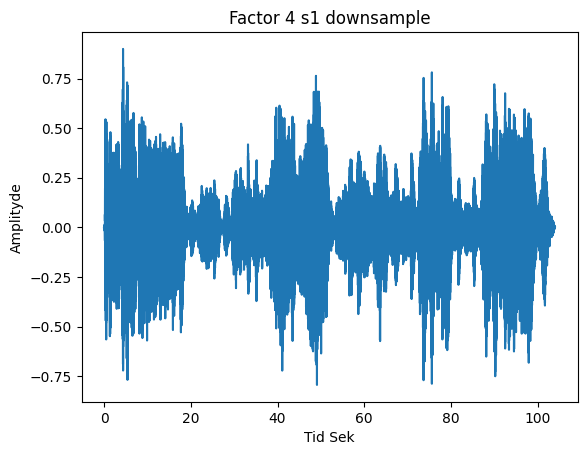
\includegraphics[width=0.8\textwidth]{images/o5_s1_dsample.png}
    \caption{Plot af signal 1 downsamplet}
    \label{fig:o5_s1_dsample}
\end{figure}
\begin{figure}[H]
    \centering
    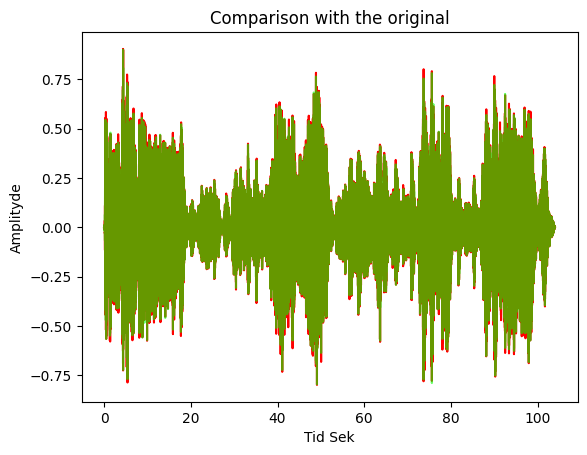
\includegraphics[width=0.8\textwidth]{images/o5_s1_compare_dsample.png}
    \caption{Plot af signal 1 sammenligning med downsample}
    \label{fig:o5_s1_compare_dsample}
\end{figure}

\subsection{Diskussion og konklusion}
På \autoref{fig:o5_s1_dsample} kan der ikke observeres nogen tydelig ændring i signalet på plottet. Ved sammenligning med det originale signal på \autoref{fig:o5_s1_compare_dsample} kan der dog ses en mindre ændring, særligt ved de yderste amplitudespidser, hvor der kan observeres et væsentligt tab. Dette kan forklares ud fra teorien bag downsampling, da høje frekvenser kan forårsage aliasing, hvis de ikke fjernes inden downsampling.

Ved downsampling af et signal kan høje frekvenser forårsage aliasing, hvilket resulterer i uønskede udsving i det lavere frekvensområde. Dette hænger sammen med Shannons samplingssætning, som angiver, at frekvenser over halvdelen af samplingsfrekvensen, altså Nyquist-frekvensen, ikke kan repræsenteres korrekt og derfor vil blive foldet ned i det lavere frekvensområde.

For at undgå dette anvender funktionen `decimate` et lavpasfilter før downsampling. Filteret dæmper de frekvenser, som ligger over den nye Nyquist-frekvens, så de ikke efterfølgende skaber aliasing i det lavere frekvensområde. Det observerede tab ved de yderste amplitudespidser kan derfor blandt andet skyldes, at højere frekvenser er blevet dæmpet af lavpasfilteret inden downsampling.


\newpage

%opgave 6
\section{Opgave: Lyt – og beskriv forskellen mellem originalen og den nedsamplede version}

\subsection{Forberedelse}
Her vil et biblioteket blive brugt til at afspille dataen som lydfil. Resultatet ligger i bilag.

\subsection{Kode}
\begin{lstlisting}[language=Python]
#udskriv de to lidsamples så der kan høres forskel
display(Audio(audio_s1[:,0], rate=f_s))
display(Audio(downsampled_f4_s1, rate=f_s//factor))
\end{lstlisting}

\subsection{Resultat}
Bilag "Signal\_s1\_.mp3"

Bilag "Signal\_s1\_downsamplet.wav"

\subsection{Diskussion og konklusion}
Lyden i den downsamplede version er mere dæmpet, og det føles, som om man befinder sig længere væk fra musikken i stedet for at være til stede i samme rum. Den originale version lyder mere nærværende, mens den downsamplede version virker mere fjern.

Dette stemmer også overens med det forventede ved downsampling, da de højeste frekvenser går tabt. Høje frekvenser bliver generelt absorberet mere af luften end lave frekvenser, når lyden bevæger sig over længere afstande. Da disse frekvenser allerede er fjernet ved downsampling, kan det bidrage til oplevelsen af, at lyden kommer fra længere væk, som om man ikke befinder sig i samme rum som musikken.


\newpage
%opgave 7
\section{Opgave: Sammenlign de to stereo-kanaler i s2 – beskriv forskelle og ligheder}

\subsection{Forberedelse}
Da jeg ikke selv kan høre nogen forskel, vil jeg plotte de to signaler i samme graf. Her vil det venstre signal være blåt, mens det højre signal vil være rødt. Der vil blive plottet både de to lydsignaler og deres frekvensspektre for at identificere eventuelle direkte forskelle og frekvenstendenser mellem de to signaler.

Det er vigtigt ved visning af frekvensspektret at følge Shannons samplingssætning og derfor kun plotte frekvenser op til halvdelen af samplingsfrekvensen. Denne grænse kaldes Nyquist-frekvensen. Frekvenserne over Nyquist-frekvensen indeholder ikke yderligere information om det originale signal, da den anden halvdel af spektret er en spejling af den første halvdel.

\subsection{Kode}
\begin{lstlisting}[language=Python]
#plot signals 2's kanaler for sammenligning
plt.plot(t_s2,audio_s2[:,0],c="#0000ff66")
plt.plot(t_s2,audio_s2[:,1],c="#ff000066")
plt.xlabel("Tid Sek")
plt.ylabel("Amplityde")
plt.title("Comparison with the original")
plt.show()



#plot signals 2's kanalers frekvens spektrum for sammenligning
S2_left = np.fft.fft(audio_s2[:,0], int(f_s))
S2_right = np.fft.fft(audio_s2[:,1], int(f_s))

#plot
plt.figure(4)
plt.clf()
plt.plot(20 * np.log10(np.abs(S2_left)),c="#0000ff66")
plt.plot(20 * np.log10(np.abs(S2_right)),c="#ff000066")
plt.xlim(0,f_s/2)
plt.xlabel("Frekvens i Hertz")
plt.title("Comparison of frekvens spektrum")
plt.show()
\end{lstlisting}

\subsection{Resultat}
\begin{figure}[H]
    \centering
    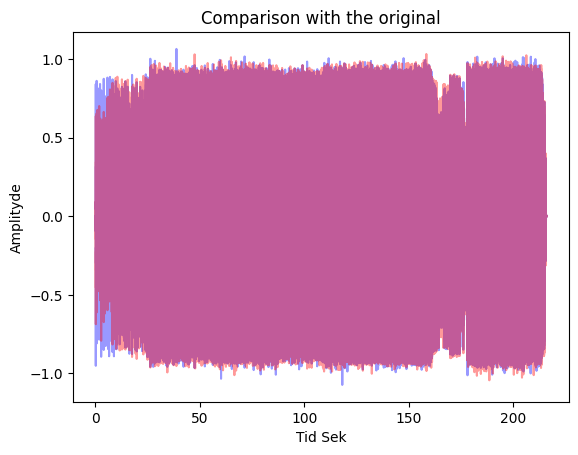
\includegraphics[width=0.8\textwidth]{images/o7_s2_sammenligning.png}
    \caption{Plot af signal 2 sammenligning af kanaler}
    \label{fig:o7_s2_sammenligning}
\end{figure}
\begin{figure}[H]
    \centering
    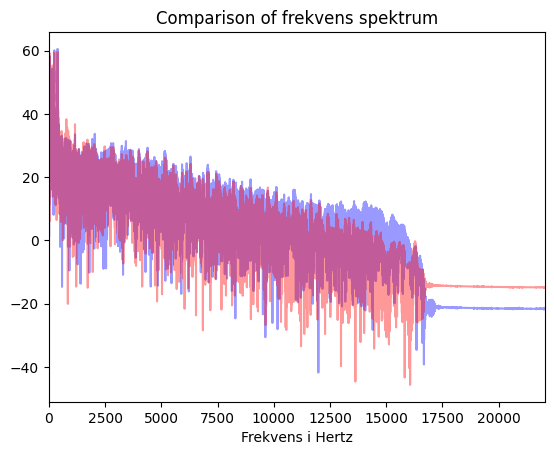
\includegraphics[width=0.8\textwidth]{images/o7_s2_spectrum_sammenligning.png}
    \caption{Plot af signal 2 sammenligning af kanaler frekvens spektrum}
    \label{fig:o7_s2_spectrum_sammenligning}
\end{figure}

\subsection{Diskussion og konklusion}
Ved en direkte sammenligning af lyden er der ikke nogen stor forskel mellem de to kanaler, hvilket forklare hvorfor jeg ikke kan høre forskel. Den tydeligste forskel ses i starten, hvor den højre kanal har en højere amplitude end den venstre kanal. Hvis vi ser på frekvensspektret for de to kanaler, kan vi også se, at de hovedsageligt indeholder de samme frekvenser. Ved en relativ sammenligning af frekvensspektrene kan det desuden ses, at den højre kanal indeholder flere høje frekvenser end den venstre kanal, særligt i området fra omkring 10 kHz til 15 kHz.

\newpage

%opgave 8
\section{Opgave: Kvantisering af s2 med 4 bit}
\subsection{Opgavebeskrivelse}
Kvantiser s2 (venstre kanal) med 4 bit (brug egen funktion eller den på BS).
Plot og lyt, - sammenlign med originalen og kommenter

\subsection{Forberedelse}
Til denne opgave vil jeg lave min egen kvantificeringsfunktion, som sigter efter at bevare amplituden så præcis som muligt. Dette inkluderer at bevare signalets maksimale og minimale amplitude og kvantificere signalet i 4 bit eller 16 niveauer mellem den maksimale og minimale amplitude.

For at udføre dette vil funktionen først finde antallet af steps, eller niveauer, ved at beregne \(2^{\text{bits}}\). Derefter vil funktionen skalere signalet, så det ligger mellem 0 og 1. Dette gøres, da signalet ikke nødvendigvis ligger mellem \(-1\) og \(1\). Ved at skalere signalet til et kendt interval bliver det muligt at tilpasse samples til de ønskede kvantiseringsniveauer.

Efter signalet er skaleret til intervallet fra 0 til 1, multipliceres signalet med antallet af steps minus 1. Dette skyldes, at værdien 0 også tæller som et step. Ved 4 bit er der derfor \(2^4=16\) niveauer, som går fra 0 til 15. Samples vil dermed have værdier mellem 0 og 15, som svarer til de 16 forskellige kvantiseringsniveauer.

Herefter afrundes værdierne til heltal, så samples placeres på et af de 16 kvantiseringsniveauer. Derefter skaleres signalet tilbage til intervallet fra 0 til 1. Til sidst skaleres signalet tilbage til det oprindelige amplitudinterval mellem den maksimale og minimale amplitude. På den måde bevares signalets oprindelige amplitudområde, mens signalet samtidig bliver kvantiseret.

I koden vil jeg desuden kontrollere, at amplitudeforholdet bevares, og at kvantiseringsprocessen ikke ændrer signalets overordnede amplitudeforhold.


\subsection{Kode}
\begin{lstlisting}[language=Python]
# få maks og min a venstre kanal
max_s2_left = np.max(audio_s2[:,0])
min_s2_left = np.min(audio_s2[:,0])

#function til at kvanticere med signalet max min og antal bits
def quantize(signal,max,min,bits):
    
    #få antallet af steps signalet skal beskrives på
    steps = 2**bits 
    
    #formater signalet til en værdi mellem 1 og 0
    maped_signal = (signal - min) / (max - min)
    
    #gang med antallet af steps for at kunne arrunde til hele tal senere
    #da 0 er en af stepsne er skal signalet kun forstærkes til værdier mellem 0 til 15
    amplified_maped_signal = maped_signal * (steps-1)
    
    #afrund til hele tal for at få signalet passet ind på de 16 steps
    steped_amplified_maped_signal = np.round(amplified_maped_signal)
    
    #divider signalet ned igen så det bliver et signal mellem 0 og 1
    steped_maped_signal = steped_amplified_maped_signal / (steps-1)
    
    #formater signalet tilbage til signales originale maks- og minimumsværdi 
    steped_signal = steped_maped_signal * (max - min) + min
    
    return steped_signal

#kvanticer signalet
q4_s2_left = quantize(audio_s2[:,0],max_s2_left,min_s2_left,4)

#check to see if amplitude is keeped
max_q4_s2_left = np.max(q4_s2_left)
min_q4_s2_left = np.min(q4_s2_left)

#pring afstanden mellem max og min før kvanticering og efter for at se om forholdet ændre sig eller om der er fejl
print(f"delta_max: {np.abs(max_s2_left-max_q4_s2_left):.3e}")
print(f"delta_min: {np.abs(min_s2_left-min_q4_s2_left):.3e}")


#plot
plotAudio("s2 Kvantiseret til 4bit",t_s2,q4_s2_left)


#plot sammenligning med originalen
plt.plot(t_s2,audio_s2[:,0],c="red")
plt.plot(t_s2,q4_s2_left,c="#00FF0099")
plt.xlabel("Tid Sek")
plt.ylabel("Amplityde")
plt.title("sammenlign bvanticering med originalen")
plt.show()

display(Audio(q4_s2_left,rate=f_s))
\end{lstlisting}

\subsection{Resultat}

\begin{lstlisting}[language=Bash]
delta_max: 0.000e+00
delta_min: 0.000e+00
\end{lstlisting}

\begin{figure}[H]
    \centering
    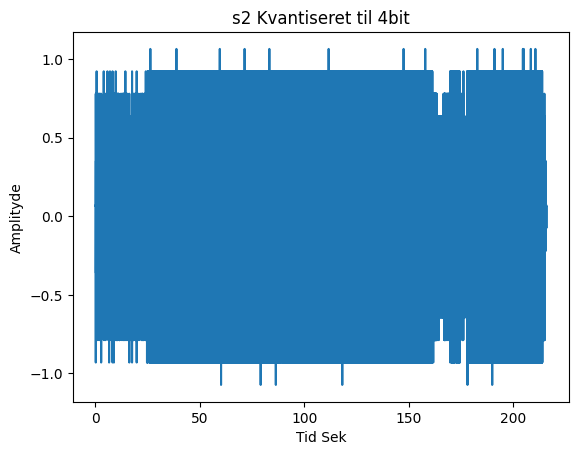
\includegraphics[width=0.8\textwidth]{images/o8_s2_4bit.png}
    \caption{Plot af signal 2 kvanticeret med 4 bit}
    \label{fig:o8_s2_4bit}
\end{figure}
\begin{figure}[H]
    \centering
    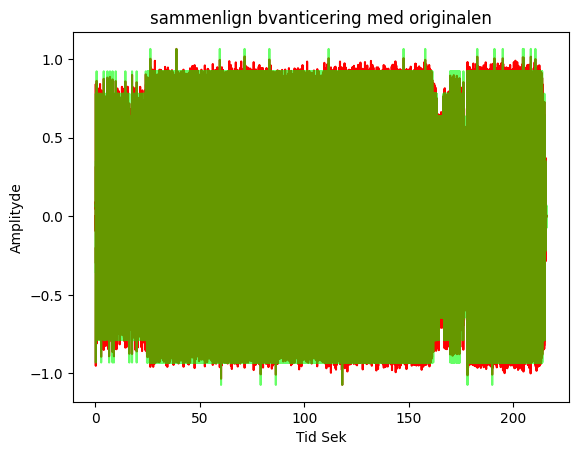
\includegraphics[width=0.8\textwidth]{images/o8_s2_4bit_compare.png}
    \caption{Plot af signal 2 kvanticering sammenligning}
    \label{fig:o8_s2_4bit_compare}
\end{figure}

Bilag "Signal\_s2\_4bit.wav"

\subsection{Diskussion og konklusion}
Den kvantiserede musik kan stadig genkendes og høres som musik, men lydkvaliteten er blevet væsentligt forringet. Der kan høres en form for statisk støj i baggrunden af hver tone, og generelt lyder det, som om musikken er præget af meget støj og forvrængning. Lyden får dermed en karakter, der minder om det, man ofte forbinder med genren *earrape*.

\newpage
%opgave 9
\section{Opgave: Fade-out på s3 med eksponentielt aftagende envelope}
\subsection{Opgavebeskrivelse}
Lav et ‘fade out’ på s3 over den sidste tredjedel med en eksponentielt aftagende envelope, hvor amplituden ved slutningen er aftaget til 5\%. Hint: Løs ligningen nedenfor og find hældningskoefficienten $\alpha$.

\subsection{Forberedelse}
Her vil jeg løse ligningen i tidsdomænet, hvor (k) er tiden, hvor lyden skal fade out, og (c) er det endelige lydniveau. Jeg vil isolere (a), så den kan beregnes i Python og bruges til at fade lyden ud.

\[
c = e^{-a(t)}
\]

Denne formel beskriver en eksponentiel aftagning, hvor værdien ved tiden 0 er \(e^0 = 1\). Aftagningen starter derfor ved 1 og falder til \(C\), når den angivne tid \(t\) er nået. Dette kan bruges til at lave en blød aftagning af lydstyrken.

Da vi i vores tilfælde ønsker, at fade-out'et skal foregå over den sidste tredjedel af lydfilen, hvor lydniveauet skal falde til 5 \%, vil værdierne være \(c = 0,05\) og \(t = \frac{1}{3}\) af lydfilens samlede tid.

Da vi ønsker at fade den sidste tredjedel af signalet ud, skal aftagningen først begynde ved to tredjedele af lydsignalets samlede længde. Derfor trækkes de første to tredjedele af tiden fra, så aftagningen starter ved \(t=0\) og når \(c\) præcis ved slutningen af lydfilen.

Hvis funktionen anvendes på hele signalet, vil lydfilen blive forstærket i perioden frem til to tredjedele af lydfilen. Derfor skal ligningen kun anvendes på den sidste tredjedel af lydfilen. Til dette findes indekset, hvor den sidste tredjedel begynder, så kun disse samples påvirkes af ligningen.

Aflede a:

\[
c = e^{-a(t)}
\]

\[
\ln(c) = -a(t)
\]

\[
\frac{\ln(c)}{t} = -a
\]

\[
a = -\frac{\ln(c)}{t}
\]


\subsection{Kode}
\begin{lstlisting}[language=Python]
audio_s3, fs_s3 = sf.read("./Signal_s3.mp3")

#find slutningstiden af lydfilen
t_end_s3 = t_s3[-1]

#beregning
#c=e^(-a(t))
#ln(c)=-a(t)
#ln(c)/(t)=-a
#a=-ln(c)/(t)
a = -np.log(0.05)/(t_end_s3/3)


#lav ny var til fade
fade_s3 = 0
fade_s3 = audio_s3[:,0]

#find index for hvor fade skal indsættes og starte fra
i_2of3_s3 = (len(fade_s3)*2)//3

#lav fadeout med formelen, formelen er regnet ud fra starten 0 til 1/3 af tiden, derfor skal tiden hvor fadeout starter trækkes fra den aktuelle tid
fade_s3[i_2of3_s3:] = np.exp(-a*(t_s3[i_2of3_s3:]-t_s3[i_2of3_s3]))*fade_s3[i_2of3_s3:]

#plot lyden
plotAudio("original",t_s3,audio_s3)
plotAudio("fadeout",t_s3,fade_s3)

display(Audio(fade_s3,rate=f_s))
\end{lstlisting}

\subsection{Resultat}
\begin{figure}[H]
    \centering
    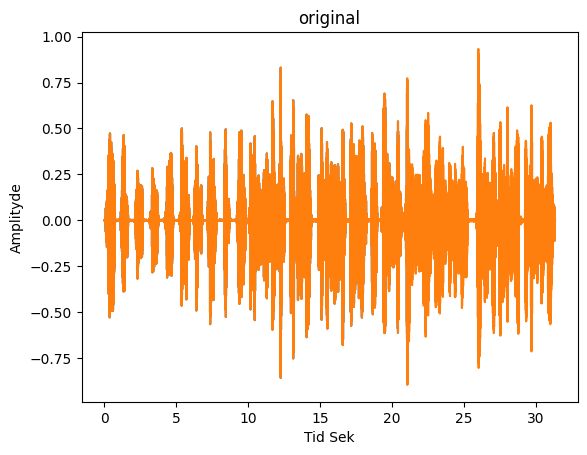
\includegraphics[width=0.8\textwidth]{images/o9_s3_original.png}
    \caption{Plot af signal 3}
    \label{fig:o9_s3_original}
\end{figure}
\begin{figure}[H]
    \centering
    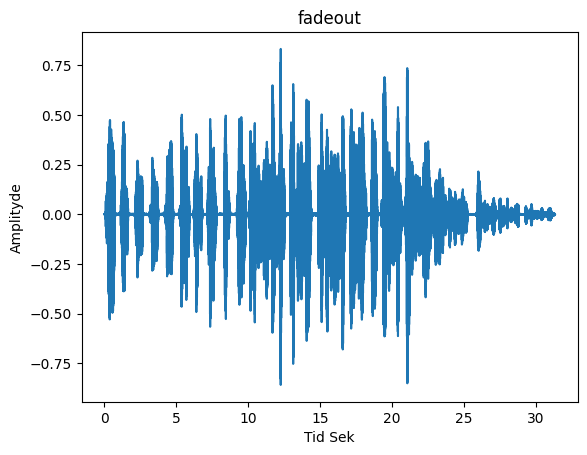
\includegraphics[width=0.8\textwidth]{images/o9_s3_fadout.png}
    \caption{Plot af signal 3 fadeout}
    \label{fig:o9_s3_fadout}
\end{figure}

Bilag "Signal\_s3\_fadeout.wav"

\subsection{Diskussion og konklusion}
I plottet på \autoref{fig:o9_s3_fadout} kan vi tydeligt se, at lydfilen med fade har en reduceret amplitude i slutningen af lydfilen sammenlignet med den originale på \autoref{fig:o9_s3_original}. Vi kan også ud fra plottet observere, at den følger den eksponentielle envelope, som vi forventer. Dette kan også tydeligt høres i lydfilen, som fader ud i den sidste tredjedel.

\newpage

\section{Opgave 10: Lav en ny udgave af s3, hvor der er et enkelt ekko med et delay på 100ms.}

\subsection{Forberedelse}
For at lave echo vil jeg først kopiere lydsamplesene over i et nyt array, hvorefter jeg vil tilføje samplesene igen, men forskudt fra de oprindelige samples. Dette vil få lydsignalet til at køre to gange, men forskudt, hvilket skaber en echo-effekt. For at få det til at lyde mere som et echo vil den forskudte lyd blive reduceret med 80 %, så kun 20 % af lyden bliver tilføjet.

For at lave offsettet vil de 100 millisekunder blive divideret med tiden mellem hvert sample. Dette giver antallet af indexes, som det ekkoede signal skal forskydes med.

\subsection{Kode}
\begin{lstlisting}[language=Python]
#indlæs lydfilen
audio_s3, fs_s3 = sf.read("./Signal_s3.mp3")

#lav en var til at holde lyden med ekko
ekko_s3 = audio_s3[:,0].copy()

#find index offset for hvor mange indexes er mellem den aktuelle lyd til at der kommer ekko
i_ekko_100ms = (int)(0.1//t_s)

#tilføj ekko, dog dempet for at få det til at lyde som reel ekko
ekko_s3[i_ekko_100ms:] += audio_s3[:-i_ekko_100ms,0]*0.2


display(Audio(ekko_s3,rate=f_s))
\end{lstlisting}

\subsection{Resultat}

Bilag "Signal\_s3\_ekko.wav"

\subsection{Diskussion og konklusion}
På lydfilen kan der tydeligt høres, at lydsignalet går igennem to gange forskudt, hvor ekkosignalet anden gang er reduceret. Det lyder, som om optagelsen er foregået i et lille rungende rum med dårlig lydabsorbering.

\end{document}